\documentclass[10pt,twocolumn]{article} %twocolumn
\usepackage{graphicx}
%opening
\title{Introduction to Supersingular Isogeny Diffie-Hellman}
\author{Pedro Miguel Sosa}

\begin{document}

\maketitle

\begin{abstract}
This paper aims to give researchers an approachable introduction to the Supersingular Isogeny Diffie-Hellman key exchange (SIDH-KEX). SIDH is one of the few post-quantum key exchange algorithms based on elliptic curves that has shown potential due to its small key sizes and quick timing. This paper will briefly describe the history and motivation of SIDH. Furthermore, we will present a simple construction of the algorithm along with the mathematical background needed to understand it. Lastly, we will present the recommended parameters to use for potential implementations.
\end{abstract}

\section{Background}
As studies in the area of quantum computing seem to yield promising results, cryptography researchers are seeking new cryptosystems that could withstand attacks from such machines. While quantum computers do not affect secret key cryptography as much\footnote{It is enough for most secret key cryptographic schemes to increase their key sizes to provide protection against quantum adversaries.}, most of the popular public key cryptosystems become vulnerable \cite{bernstein2009introduction}. 
\par Most popular public key cryptosystems used today rely on the hardness of the factorization problem. For classical machines, the best known attacks would take exponential time, however, quantum computers are able to do factoring in polynomial time using Shor's algorithm.
\par As a result, there has been an important push towards the study and implementation of Post-Quantum cryptographic protocols in these past few years. This has yielded many different Post-Quantum Cryptographic (PQC) schemes based on lattices, codes, hashes, multivariate equations, and most recently elliptic curves.
\par This paper will focus on Supersingular Isogenies Diffie-Hellman (SIDH), which is the one of the few PQC algorithm based on elliptic curves. It was created in 2011 by De Feo, Jao and Plut \cite{Jao2011} and has since been implemented and optimized by others. In 2016, researchers at Microsoft published a version of SIDH which ran in constant time and used public keys of size 564 bytes, showing that SIDH had ``strong potential as a PQC candidate"\cite{costello2016}.

\section{Security and Efficiency}
\paragraph{Security} Although both ECDH and SIDH use elliptic curves, their underlying problem is different. ECDH's hardness rests upon the discrete logarithm problem, whereas SIDH's hardness rests up the difficulty of finding the isogeny mapping between two supersingular elliptic curves with the same number of points. 
\par It has been proven \cite{delfs2016computing,biasse2014quantum} that SIDH's security against classical computers is $O(p^\frac{1}{4})$, while the security against quantum computers has been theorized to be  $O(p^\frac{1}{6})$.
\paragraph{Efficiency} SIDH has become substantially more efficient since its release in 2011. The latest implementations published in 2016 runs in constant time and has a public key size of 564 bytes. This key size is among the smallest in comparison to other PQC key exchange alternatives. This latest implementation has been added to the Open Quantum Safe's ``OpenSSL" project to be used for Internet applications \footnote{Repository: github.com/open-quantum-safe/openssl}.

\begin{figure}[t]
	\centering
	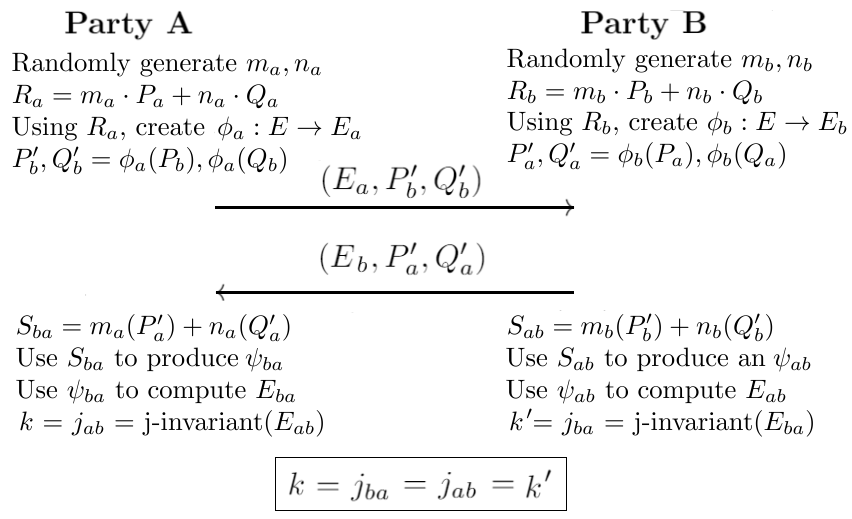
\includegraphics[width=1.02\linewidth]{sidh}
	\caption{Visual Representation of SIDH-KEX}
	\label{fig:sidh}
\end{figure}

\section{Preliminaries}

In this section we will discuss some of the mathematical constructs and finer details necessary to further understand the SIDH-KEX.

\paragraph{Elliptic Curves}
Similar to other elliptic curve cryptographic schemes, we will assume our chosen elliptic curve $E$ over $F_{p^2}$ to be non-singular and of the Weierstrass form: $y^2 = x^3 + ax + b$. As such, all point addition and multiplication must be calculated by using the functions defined for these types of curves.

\paragraph{Isogeny} An isogeny is a surjective and homomorphic structure preserving function that maps two groups together. In the case of elliptic curves case, a  isogeny $\phi$ will map points on the domain curve $E$ to points on a co-domain curve $E'$. These isogenies are calculated using V{\'e}lu's formulas \cite{velu1971isogenies} as $\phi: E \rightarrow E/\kappa$, where $\kappa$ is defined as the kernel.

\paragraph{j-Invariant}
The j-invariant is a descriptor that can be computed for any particular curve using said curves parameters. Most importantly, isomorphic curves will always share the same j-invariant value. The exact equation for the j-invariant will vary depending on the underlying form of the elliptic curve. In the case of elliptic curves in the Weierstrass form, the j-invariant is calculated as follows:

\begin{center}
	\centering
	$j(E)=1728\cdot\frac{4a^3}{4a^3+27b^2}$
\end{center}




\paragraph{Supersingular curves} While it might seem a bit confusing, supersingular curves are non-singular elliptic curves as one would expect to find in other elliptic curve scheme. The term \textit{``supersingular}" actually refers to the fact that they have ``singular" values of the j-invariant and its Hasse invariant is 0. Refer to section \ref{sec:params} for a concrete curve suggestion.

\section{Supersingular Isogeny Diffie-Hellman}
Intuitively, the SIDH key exchange works by having both parties generate a secret key, which will be an isogeny based on the known public curve $E$ and points $P_a,Q_a,P_b,Q_b$ (which reside on $E$). Then each party will create and exchange a new curve derived from their secret isogenies. This new curves can be considered the ``public keys". Afterwards, by merging their ``private key" isogenies and the other party's ``public key" curve, each party will be able to generate a final curve. For both parties, these final curves will have the same j-invariant (since they are isogenous with respect to each other). As such the value of this j-invariant becomes the shared secret.



\subsection{Public Parameters}
Initially there will be 4 global public parameters:
\par - A prime $p$ 
\par - A supersingular elliptic curve $E$ over $F_{p^2}$
\par - Four fixed points $P_a,Q_a,P_b,Q_b$ on $E$ 


\subsection{Key Exchange}

- \textbf{Party A} 
\newline
1. Randomly generate $ m_{a},n_{a}$
\newline
2. $R_{a} = [m_{a}]P_{a}+[n_{a}]Q_{a}$
\newline
3. $\phi_{a}: E \rightarrow E_{a} = E/\langle R_{a}\rangle$
\newline
4. $P'_{b},Q'_{b}=\phi_{a}(P_{b}),\phi_{a}(Q_{b})$
\newline
5. Send $(E_{a}, P'_{b}, Q'_{b})$ to Party B
\newline
6. Receive $(E_b, P'_a, Q'_a)$ from Party B
\newline
7. Calculate $S_{ab} = [m_a]P'_a+[n_a]Q'_a$ 
\newline
8. $\phi_{ab}=E_{a}\rightarrow E_{ab} = E_{a}/ \langle S_{ab} \rangle $.
\newline
9. Compute $k$ = $j_{ab}$ = j-invariant($E_{ab}$)
\newline
\newline
- \textbf{Party B}
\newline
1. Randomly generate $ m_{b},n_{b}$
\newline
2. $R_{b} = [m_{b}]P_{b}+[n_{b}]Q_{b}$
\newline
3. $\phi_{b}: E \rightarrow E_{b} = E/\langle R_b\rangle$
\newline
4. $P'_{a},Q'_{a}=\phi_{b}(P_{a}),\phi_{b}(Q_{a})$
\newline
5. Send $(E_{b}, P'_{a}, Q'_{a})$ to Party A
\newline
6. Receive $(E_a, P'_b, Q'_b)$ from Party A
\newline
7. Calculate $S_{ba} = [m_b]P'_b+[n_b]Q'_b$ 
\newline
8. $\phi_{ba}=E_{a}\rightarrow E_{ba} = E_{b}/ \langle S_{ba} \rangle $.
\newline
9. Compute $k'$ = $j_{ba}$ = j-invariant($E_{ba}$)
\newline



\par Notice that since both curves are isogneous to each other, they will have the same j-invariant. As such, the shared key $k$ calculated by both parties will be the same.




\subsection{Parameter Selection}
\label{sec:params}
The latest work by Costello et al. \cite{costello2016}, defined the curve $E = y^2+x^3 +x$ and the prime $p = 2^{372}\cdot 3^{239}-1$. Furthermore they established the four points on $E$ to be: \\
- $P_{a} = [3^{239}](11,\sqrt{11^3+11})$ \newline
- $Q_a=\tau(P_a)$ \newline
- $P_b=[2^{372}](6,\sqrt{6^3+6})$ \newline
- $Q_b=\tau(P_b)$ \newline
where $\tau$ is a distortion map from $E(F_{p^2})\rightarrow E(F_{p^2}) : (x,y) \rightarrow (-x,iy)$. This was done purposely so as to avoid having to store both $Q_a$ and $Q_b$ in memory and instead derive them from their respective $P_i$ points.

\section{Future Work}
While SIDH seem very promising, there are still some issues that remain to be solved. Current implementations assume both parties are honest peers, and thus, an misbehaving/attacking party could leak information and weaken then security of the scheme. Another issue is the lack of crypto-analitic research done for this scheme, as the literature in which one can rely is rather limited.
\par Being a relatively new field, there are still many unknowns as to what supersingular isogenies can also be used for. Aside from key exchange, some researchers have also worked on applying supersingular curves to build digital signature schemes \cite{jao2014isogeny,sun2014toward}. 
\par However, with the recent promising developments in SIDH, work with supersingular curves is bound to gather more research in the upcoming years. 




\bibliographystyle{ieeetr}
\bibliography{main}


\end{document}

